\documentclass[11pt]{article}

\usepackage[french, english]{babel}

\usepackage[T1]{fontenc}

\usepackage{amsfonts}
\usepackage{amsmath}
\usepackage{amssymb}

\usepackage{graphicx}
\usepackage{multirow}
\usepackage{multicol}
\usepackage{xcolor}
\usepackage[shortlabels]{enumitem}

\usepackage[margin=2cm]{geometry}

\usepackage{mathtools}
\usepackage{siunitx}
\usepackage{braket}

\usepackage{listings}
\renewcommand\lstlistingname{Code Python}

\lstset{frame=tb,
  language=Python,
  numbers=left,
  stepnumber=1,
  aboveskip=3mm,
  belowskip=3mm,
  showstringspaces=false,
  columns=flexible,
  basicstyle={\small\ttfamily},
%   numbers=none,
  numberstyle=\tiny\color{gray},
  keywordstyle=\color{blue},
  commentstyle=\color{paired2b},
  stringstyle=\color{paired3b},
  breaklines=true,
  breakatwhitespace=true,
  tabsize=1,
  frame=single,
%   showtabs=false,
}


\begin{document}


\hrule

\begin{center}
  {\Large GEI299 - Gestion de projet} \\ \vspace{5mm}
  {\LARGE\sffamily Devoir 1} \\
  Alexis Jean \\
  À remettre le 25 septembre
\end{center}

\hrule


\section{\underline{Introduction au contrat}}
Le client M. Scanner de la compagnie GE Healthcare souhaite explorer les possibilités de différents métaux pouvant être utilisés comme agent de contraste dans les images de résonance magnétique (IRM). La raison, l'agent de contraste en utilisation actuelle, le gadolinium, est trop toxique pour le client. Ce dernier requiert de notre expertise pour développer un logiciel pouvant sélectionner un candidat de remplacement parmi différents critères choisis par le client.


\section{\underline{Éléments à inclure, contraintes et points à clarifier}}

\subsection{Éléments à inclure}
Dans la section qui suit, les éléments à inclure ainsi que les contraintes du client seront présentés sous forme de deux listes de puces. Selon les demandes du client, il nous faudra apporter les fonctionnalités suivantes comme nécessité au produit qui est demandé :

\begin{itemize}[label=\textbullet]
  \item Une interface utilisateur simple et intuitive aux couleurs de GE Healthcare
  \item Le logiciel doit permettre l'ajout, la modification et la suppression de métaux de la base de données jugés comme candidats potentiels
  \item Un module de simulation quantique (via la plateforme de IBM) doit être intégré pour pouvoir calculer l’état fondamental et les propriétés électroniques des complexes métal-ligand
  \item Une façon de pouvoir comparer les différents candidats selon différents critères
  \item Avoir la possibilité de pouvoir exporter les résultats sous différents formats
  \item Le logiciel doit avoir deux modes : un mode scientifique et un mode affaires
\end{itemize}

\subsection{Contraintes}
Le client a aussi des contraintes qui viennent avec sa demande qui se listent telles que :

\begin{itemize}
  \item Le logiciel doit être compatible avec autant Windows que MacOS
  \item Le temps de calcul pour une simulation standard doit être inférieur à 2 minutes et d'avoir un taux d'erreur inférieur à 2\%
  \item Un langage et un framework maintenable avec une connexion sécurisée à la plateforme IBM Quantum pour l’exécution des calculs sont nécessaires
  \item Le budget maximal permis est de 200 000\$ qui couvre le matériel quantique, les ressources humaines ainsi que le matériel
  \item Le produit final doit être livré au bout de 2 mois mentionnés
  \item Le code doit être modulaire pour des ajouts et doit posséder un plan de maintenance sur 12 mois
\end{itemize}

\subsection{Points à clarifier}
Dans l'analyse de l'énoncé, quelques questions ont été retenues qui doivent être communiquées avec le client pour la bonne continuation du projet. Comme précédemment, les questions seront énoncées sous forme de liste de puces :

\begin{itemize}
  \item Quel est le niveau de détail qui est attendu pour le mode scientifique du logiciel ?
  \item Pour pouvoir comparer les taux d'erreur, comment pouvons-nous obtenir la référence classique ?
  \item Pour ce qui est de l'interface, y'a-t-il une préférence pour le web ou desktop ?
\end{itemize}
Voici un exemple de réponse possible pour chaque question :

\begin{itemize}
  \item Le mode scientifique doit apporter des graphiques, des calculs complets ainsi qu'un rapport complet de chaque simulation
  \item Les références classiques se trouvent dans l'échantillon en pièce jointe dans le matériel du projet
  \item Une interface desktop sera préférée pour aider à la sécurisation des résultats directement sur les machines de la compagnie
\end{itemize}


\section{\underline{Diagramme d'entrées/sorties du logiciel}}
Comme stipulé dans le contrat du client, un diagramme des entrées et des sorties est demandé. Voici alors le diagramme :

\begin{figure}[h!]
  \includegraphics[width=\linewidth]{diagramme.png}
  \caption{Diagramme entrées/sorties}
\end{figure}
\pagebreak


\section{\underline{Aperçu de l'interface du logiciel}}
Comme prévu dans l'entente avec le client, un aperçu de l'interface utilisateur du logiciel est fourni dans le cahier de spécification des exigences. Voici la dite interface :

\begin{figure}[h!]
  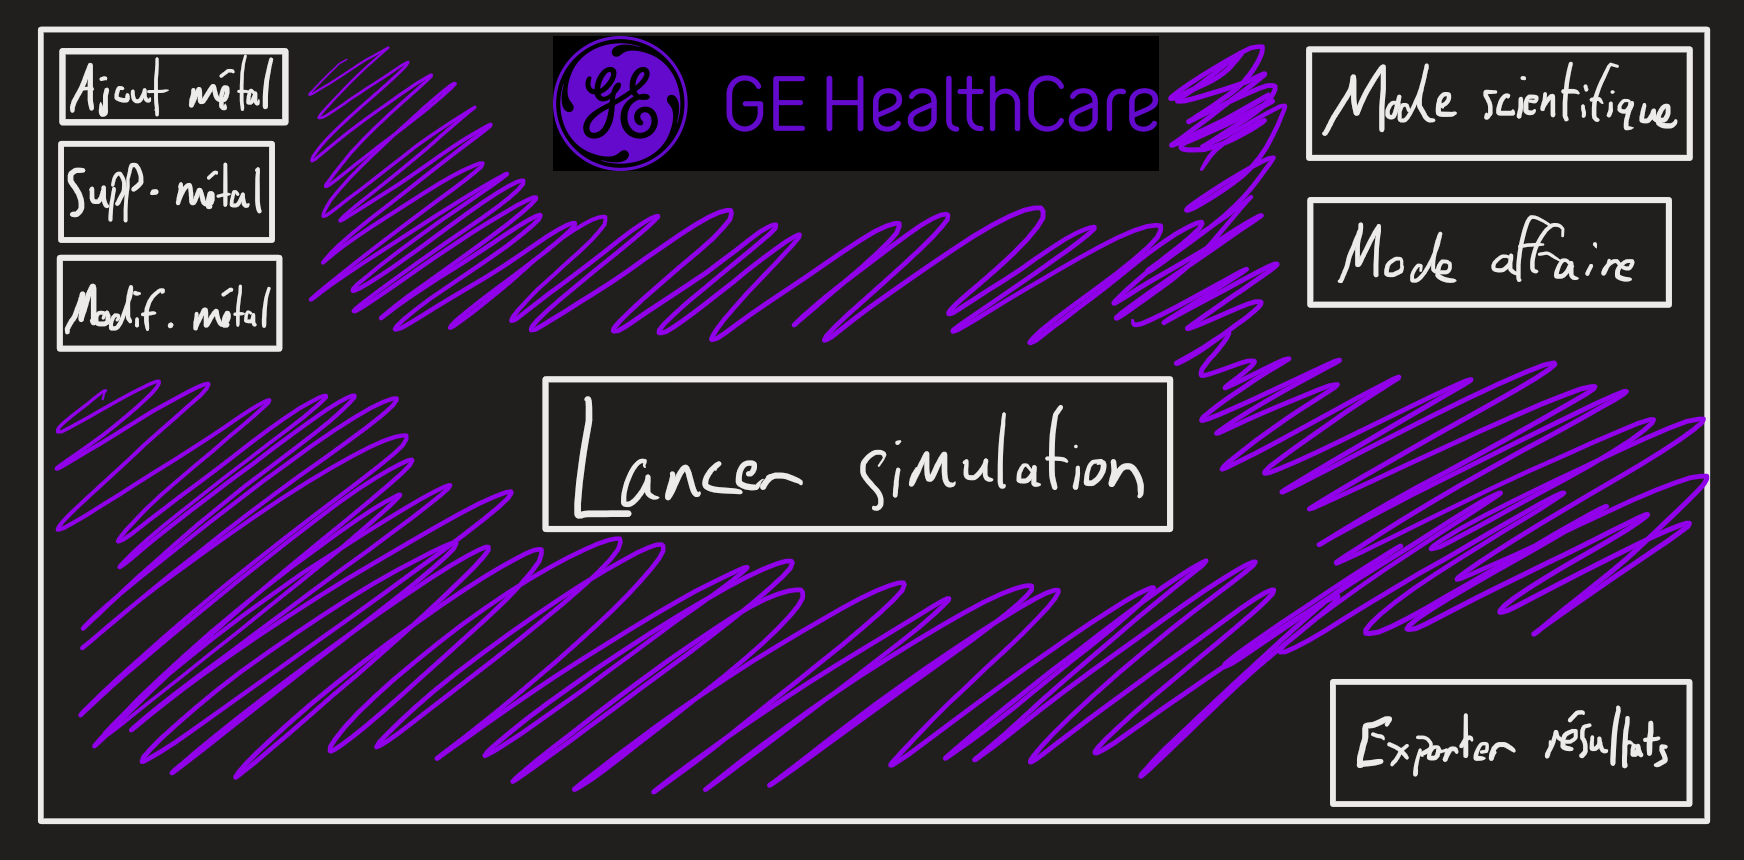
\includegraphics[width=\linewidth]{interface.png}
  \caption{Aperçu de l'interface du logiciel (représentation d'artiste)}
\end{figure}

\subsection{Légende de l'interface}
Maintenant, toutes les fonctionnalités de l'interface seront décrites en allant de gauche à droite et de haut en bas :

\begin{itemize}
  \item Ajout métal : Ce bouton sert à ajouter un métal candidat pour la simulation
  \item Supp. métal : Ce bouton sert à retirer un métal candidat de la simulation
  \item Modif. métal : Ce bouton sert à modifier le métal candidat actuel par un autre candidat
  \item Lancer simulation : Ce bouton sert à lancer la simulation
  \item Mode scientifique : Ce bouton sert à passer en mode scientifique pour les résultats de la simulation
  \item Mode affaire : Ce bouton sert à passer en mode affaire pour les résultats de la simulation
  \item Exporter résultats : Ce bouton sert à exporter les résultats. Lorsque cliqué, un menu apparaît pour demander le format dans lequel les résultats seront exportés
\end{itemize}
\pagebreak


\section{\underline{Attributs fonctionnels et non-fonctionnels}}
Cette section traite des attributs fonctionnels et non-fonctionnels du logiciel. Ces derniers seront émis sous forme de deux listes de puces. En premier lieu, les attributs fonctionnels :

\begin{itemize}
  \item La gestion des métaux tel que l'ajout, la suppression ou la modification avant de lancer la simulation
  \item Le classement des métaux selon les différents critères choisis par la compagnie
  \item La simulation quantique en soit, elle est initialisée par l'utilisateur
  \item L'exportation des résultats sous différents formats
\end{itemize}
Ensuite, voici les attributs non-fonctionnels du logiciel :

\begin{itemize}
  \item La vitesse des calculs ainsi que le taux d'erreur par rapport à la référence classique
  \item La sécurité avec la plateforme IBM quantique
  \item La modularité du code du logiciel
  \item La possibilité du logiciel de pouvoir être utilisé autant sur Windows que sur MacOS
\end{itemize}


\section{\underline{Besoins conflictuels}}
Les besoins conflictuels seront identifiés à l'aide d'une matrice de corrélation, puis, elle sera suivi par un court texte qui identifie où se trouve les corrélations.

\begin{figure}[h!]
  \centering
  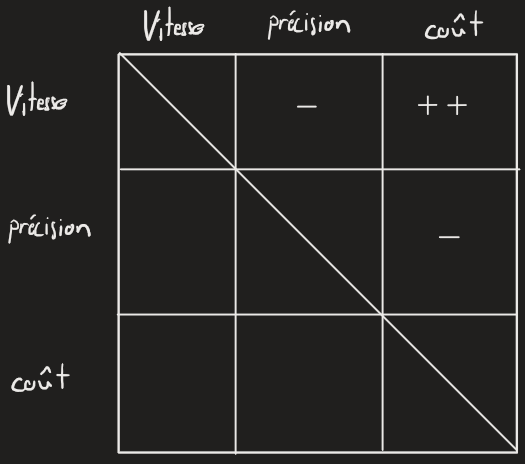
\includegraphics[scale=0.5]{matriceCorrelation.png}
  \caption{Matrice de corrélation (représentation d'artiste)}
\end{figure}
Si la vitesse est priorisée, la précision sera sacrifiée pour que le temps de calcul soit moins cher sur la plateforme de IBM. Pour la précision, si elle est priorisée, alors il va nécessairement falloir que le temps de calcul soit plus long et donc, que cela coûte plus cher d'utilisation.
\pagebreak


\section{\underline{Ébauche du manuel d'utilisation}}
En premier lieu, l'utilisateur ouvre le logiciel et arrive sur l'interface illustrée plus tôt. Il va sélectionner un métal parmi la base de données de la compagnie ainsi qu'un ligand en même temps. En deuxième lieu, une fois que tout a été choisi pour une simulation, l'utilisateur va lancer la simulation à l'aide du bouton approprié, puis, il patiente le temps que la simulation se fait sur la plateforme de IBM. Une fois que la simulation est terminée, l'utilisateur choisit le mode qui lui convient et exporte les résultats dans le format de son choix.


\section{\underline{Énoncé du problème}}

\begin{itemize}
  \item \underline{Contexte}\\Dans les IRM, des agents de contrastes sont utilisés, cependant, ils sont à base de gadolinium qui est toxique. Le client : GE Healthcare souhaite trouver des alternatives qui soient sûres pour les patients
  \item \underline{Ce que doit être la conception}\\Un logiciel facile d'utilisation et précis capable de faire des simulations quantiques sur la plateforme d'IBM et de comparer des métaux candidats. Le coût ne doit pas dépasser 200 000\$ et doit être livré en 2 mois.
  \item \underline{Livrables}\\Un logiciel étant compatible avec Windows et MacOS et associé avec ce dernier : un rapport technique, un cahier Jupyter ainsi qu'une présentation destinée aux hauts-dirigeants de la compagnie
\end{itemize}


\end{document}







